\chapter{Implementation}
\label{chap:implementation}

To achieve the most precise results it was necessary to run different scanners multiple times. JSON reports had to be then manually parsed to extract the data on a number of occassions. In order to automate this process and develop an application that would vastly improve the monitoring possibilities inside a Kubernetes cluster, we needed a tool that aggregates multiple scanners into one solution, automatically parses the results and visualizes them. Thus, KSA dashboard has emerged, comrised of the three components, two backend ones and one frontend: \textbf{ksa-aggregator}, \textbf{ksa-parser} and \textbf{ksa-dashboard}, respectively. Since the microservices are developed specifically for the Kubernetes environment and need to be closely integrated with it, Go was chosen as the primary language for the backend microservices. ReactJS was chosen for the frontend as one of the simplest yet very powerful JavaScripts frameworks (though we used Typescript). This chapter focuses on some of the implementation aspects of the KSA Dashboard. 

\section{Architecture and Software Design}
\label{sec:architecture}

Architecturally, the software product is comprised of three components. As shown on the schematic overview of the deployment (Fig~\ref{img:ksa-schematic-overview}), these components use HTTP API requests and Websockets for the communication. We can safely use unprotected HTTP protocol without TLS as the components are deployed inside one namespace and use internal communication channels only. We use websockets to notify frontend of events on the backend, which makes frontend very responsive, but tightly couples these components. A message queuing system like Kafka or RabbitMQ was considered as an alternative solution that would loosen the components and make them less dependant on each other, but it was decided against it as the system is not very big and messaging does not occur too often. Using message broker would only add extra complexity to the solution in our case.

From the feature perspective, the tool was designed to help DevSecOps engineer manage Kubernetes secuirty and, thus, serves the following requirements:
\begin{itemize}[noitemsep]
    \item User must be able to trigger the scan from the dashboard.
    \item Scanning and parsing should occur automatically without user interaction.
    \item Scan results should be persisted in the database for the future use.
    \item User must be able to browse the scan results.
    \item User must be able to search through the results.
    \item User must be able to generate reports based on the scan results.
    \item User must be able to manipulate findings (delete or mark as resolved).
    \item Dashboard should provide the possibility to be extended with other security scanners in the future.
    \item Dashboard should be able to generate graphic visualisation of the scan results.
\end{itemize}

The component diagram on the Fig~\ref{img:ksa-component-diagram} illustrates the architecture of a Kubernetes-native security scanning system. The process begins with the Dashboard component, which allows users to trigger scans and query results. Scan requests are forwarded to the Aggregator, which continues the process by initiating and watching for the scan job through the Kubernetes API. The Kubernetes API is responsible for scheduling the execution of containerized scanner jobs (such as Trivy, Kube-bench, and Prowler) within the cluster. Once the scanners complete their tasks, Aggregator component initiates parsing by sending a request to the Parser component, results are then stored in the Database component, which supports query operations for both the Dashboard and Aggregator. Additionally, the Parser exposes a WebSocket endpoint that enables real-time updates to the Dashboard—notifying it asynchronously when scan results are available. This decoupled, event-driven approach improves system responsiveness and user experience.

\begin{figure}[!hbt]
	\begin{center}
		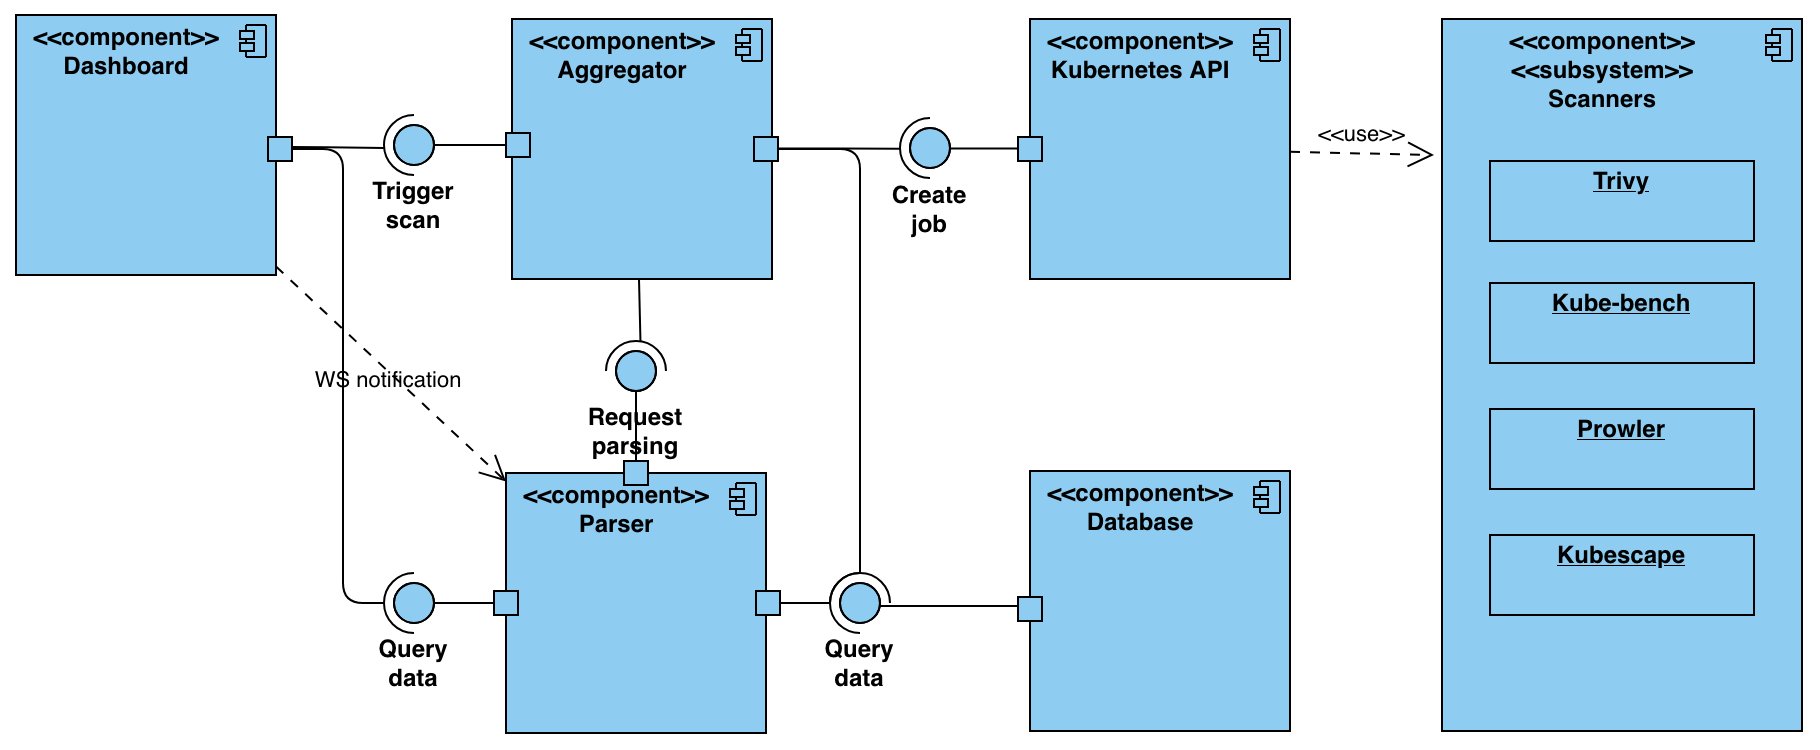
\includegraphics[width=0.9\textwidth]{images/ksa-component-diagram.png}
        \caption{Component diagram of the dashboard.}
		\label{img:ksa-component-diagram}
	\end{center}
\end{figure}

As seen on the Fig~\ref{img:ksa-schematic-overview}, both Parser and scanner Jobs mount the same PVC, where the results of the scan are stored. Each scanner has its own PersistentVolumeClaim, so that they can perform simultaneous writing uninterrupted. Those PVCs are mounted into specific directories on the Parser pod, that reads reports created by the scan jobs from these directories.

\begin{figure}[!hbt]
	\begin{center}
		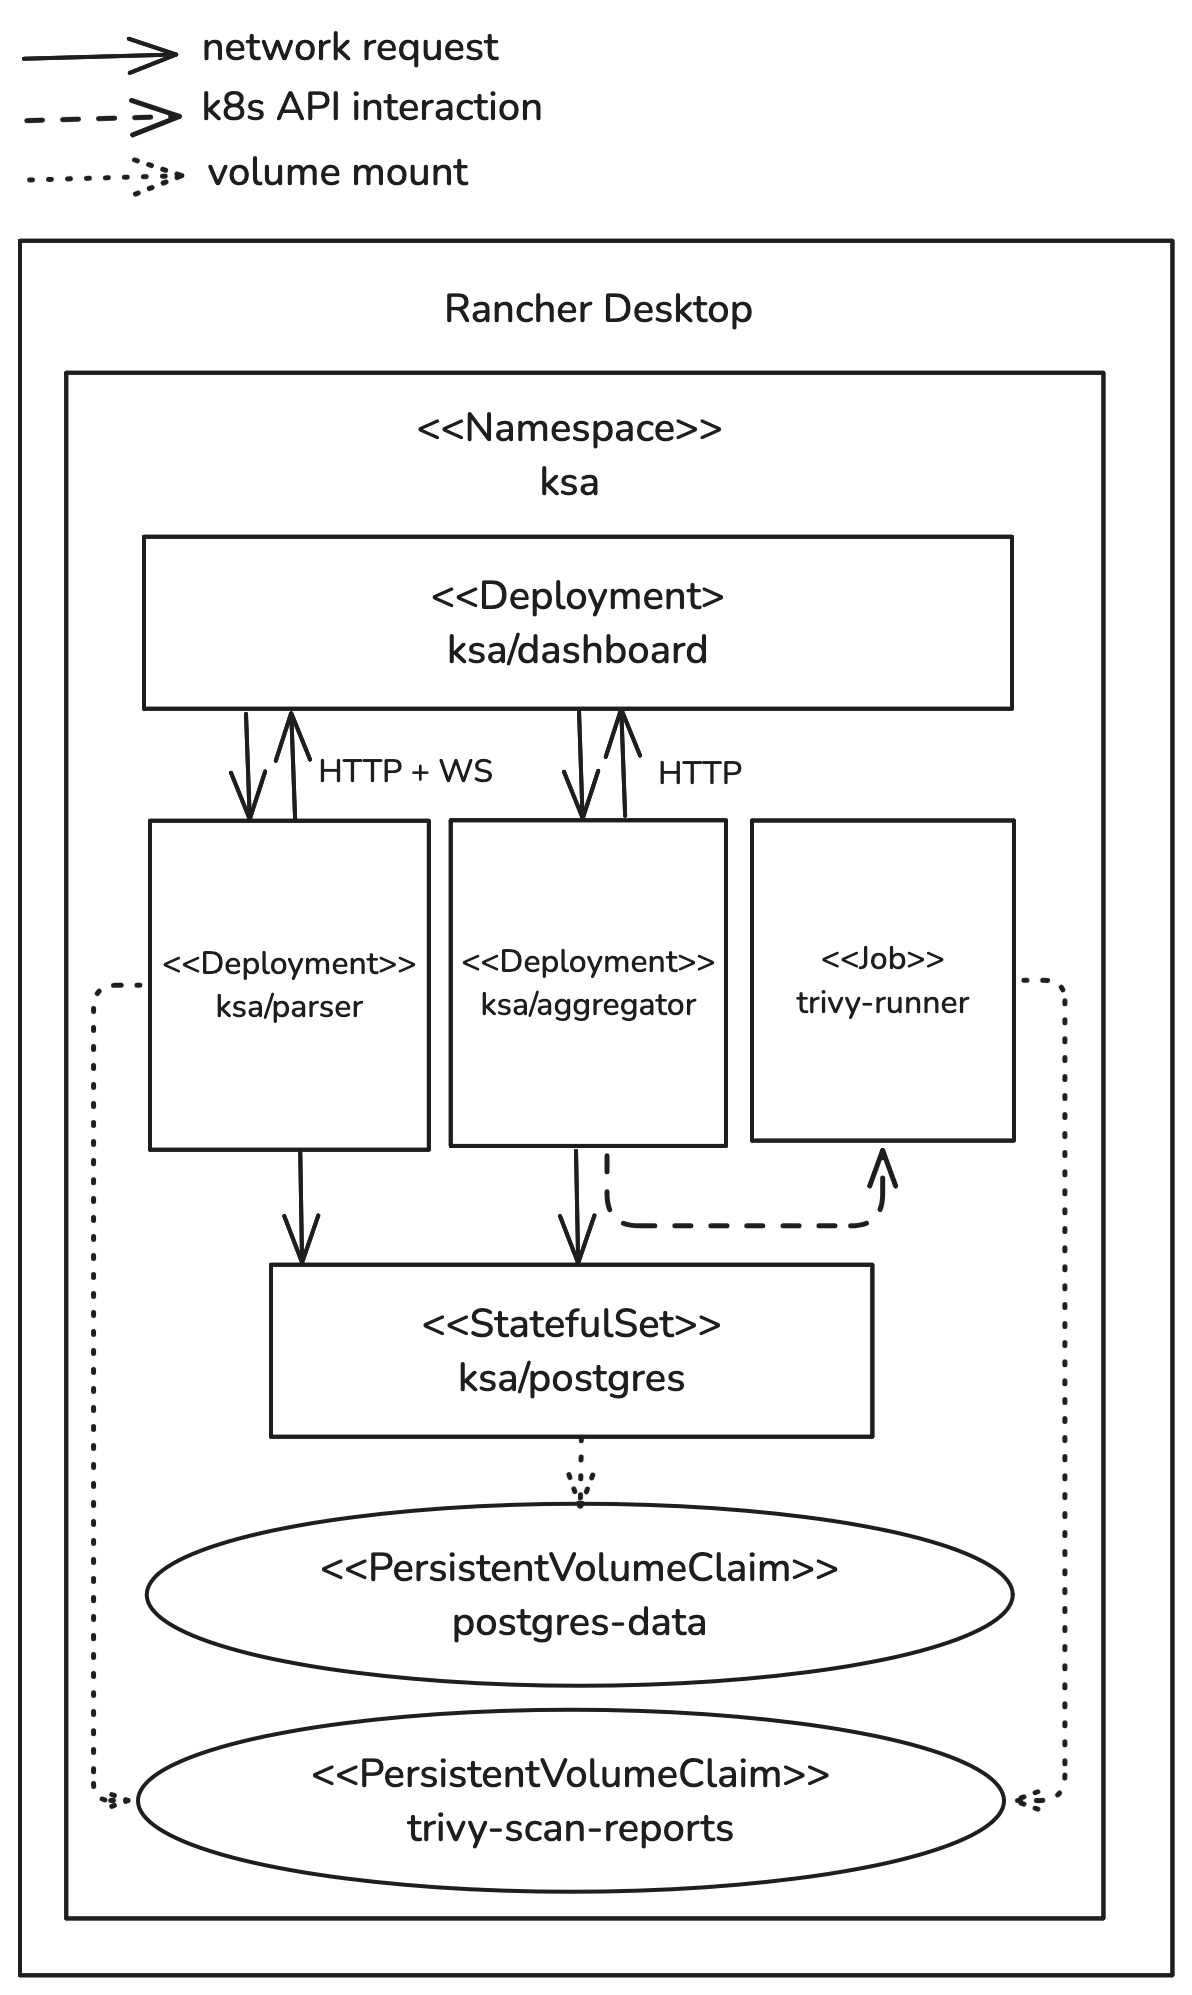
\includegraphics[width=0.5\textwidth]{images/ksa-schematic.png}
        \caption{A schematic overview of the KSA dashboard deployment.}
		\label{img:ksa-schematic-overview}
	\end{center}
\end{figure}
\section{Data Design}
\label{sec:data-design}

Data design of the solution is very simple. Table \lstinline{scanner} holds the supported scanner and its contents are constant, they do not change during runtime. Table \lstinline{report} is used to store report metadata. Tables \lstinline{vulnerability} and \lstinline{misconfiguration} store the findings extracted from the reports. Figure~\ref{img:er-diagram} depicts those entities and relationshipes between them.

\begin{figure}[!hbt]
	\begin{center}
		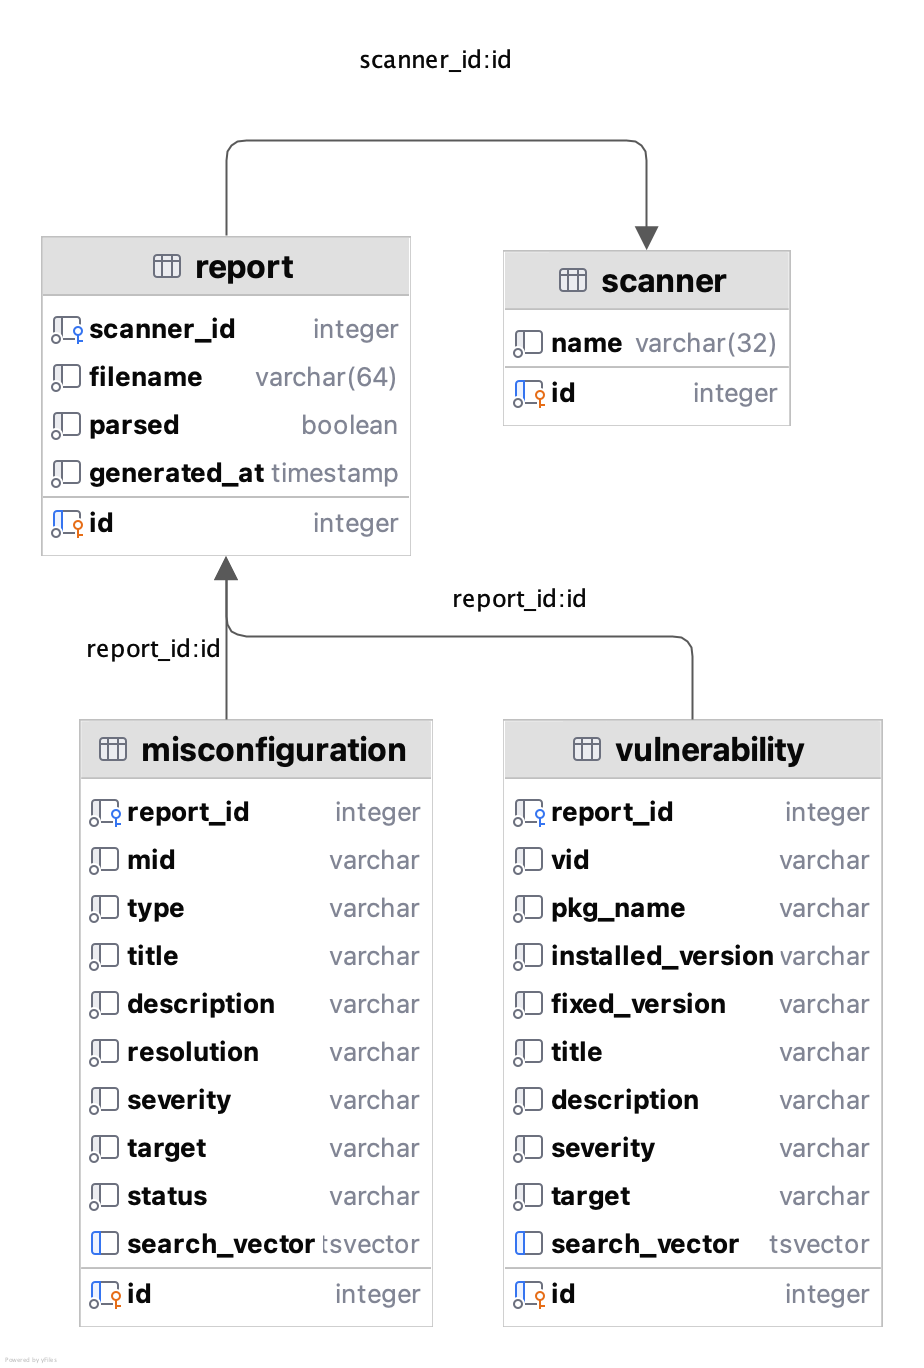
\includegraphics[width=0.5\textwidth]{images/er-diagram.png}
        \caption[Entity relationship diagram visualizing the KSA dashboard database tables and their relationship.]{Entity relationship diagram visualizing the KSA dashboard database tables and their relationship. Icons next to the column names provide necessary information about the column. Little circle in the bottom left corner depicts \lstinline{NOT NULL} constraint. Golden key denotes primary key and blue key denotes foreign key. Blue side indicates that this column is indexed.}
		\label{img:er-diagram}
	\end{center}
\end{figure}

Notice that both \textbf{vulnerability} and \textbf{misconfiguration} tables have \lstinline{search_vector} column. This column is generated when a new row is inserted or updated and used for the full-text search on these tables. Listing~\ref{lst:db-search-vector} shows the definition of the respective triggers for this column, which transform certain fields like misconfiguration id, description and title into tokens, which are then used to perform search like this: \lstinline{search_vector @@ plainto_tsquery(%s)}, where \lstinline{%s} is substitute string for the query.

\begin{lstlisting}[language=SQL, caption={[Search vector definition for misconfiguration inside the database initial script] Search vector definition for \lstinline{misconfiguration} inside the database initial script.}, label={lst:db-search-vector}]
    alter table misconfiguration 
        add column search_vector tsvector;
    create index misconfiguration_search_vector_idx on 
        misconfiguration using gin (search_vector);
    
    create function misconfiguration_update_search_vector() 
        returns trigger as $$
    begin
        new.search_vector := to_tsvector('english', new.mid ||
         ' ' || new.type || ' ' || new.title || ' ' ||
          new.description || ' ' || new.target);
        return new;
    end;
    $$ language plpgsql;
    
    create trigger misconfiguration_search_vector_trigger
    before insert or update on misconfiguration
    for each row execute function 
        misconfiguration_update_search_vector();
\end{lstlisting}
\section{Parser}
\label{sec:parser}

To make the product extendable, parser service defines a common interface for all security scanner parsers and provides a common definition of vulerabilty and misconfiguration using Golang structures. Listing~\ref{lst:parser-interface} shows a code snippet of the definition. Golang does not support objects and classes in the traditional sense. Instead, it uses interfaces: any structure that implements the methods of the interface is considered to satisfy that interface.

\begin{lstlisting}[language=Go, caption={[A common interface for parsers] A common interface for parsers.}, label={lst:parser-interface}]
    /* Parser defines a common interface 
    for all security scanner parsers */
    type Parser interface {
        Parse(filePath string) ([]Vulnerability, 
            []Misconfiguration, error)
        GetResults() interface{}
        GetVulnerabilities() []Vulnerability
        GetMisconfigurations() []Misconfiguration
    }
\end{lstlisting}

We parse the JSON reports using the standard Go module \lstinline{encoding/json}. However, the structure of those reports varies significantly and sometimes is very complex. Some reports, like the ones produced by Kube-bench for instance, are missing some fields. Kube-bench does not specify the severity of its findings, neither it specifies the target. In this case we have to use default values: we set severity to \textbf{HIGH}, for example. Additionally, Kube-bench sets status to \textbf{WARN} for manual checks and those have to be remapped onto \textbf{MANUAL} to be consistent with the Prowler's notation.

Go's \lstinline{net/http} library is used to expose a number of endpoints for other services to use. As the server creates a new goroutine for each incoming HTTP request, we have to be careful with our data. Instances of our parsers are static and shared by those goroutines. That is why each instance has a mutex, that is locked whenever a critical operation is performed on the data and unlocked afterwards.

In order to extend the Parser with a new tool, there are three things to be considered:
\begin{enumerate}[noitemsep]
    \item A new implementation of the parser interface (see Listing~\ref{lst:parser-interface}) should be defined. It must have \lstinline{Parse()} method, which would define parsing process for the scanner.
    \item This implementation should be added to the parser initialization inside the main function.
    \item Parser should be added to the database.
\end{enumerate}
\section{Aggregator}
\label{sec:aggregator}

Aggregator service defines a common interface for all security scanner runners and provides a common interface for job tracking. Listing~\ref{lst:runner-interface} shows a code snippet of the definition.

\begin{lstlisting}[language=Go, caption={[A common inteface for runners] A common inteface for runners.}, label={lst:runner-interface}]
    /* Runner defines a common interface 
    for all security scanner runners */
    type Runner interface {
        Run() error
        GetStatus() JobStatus
        CleanUp() error
        Watch(*sql.DB) (int, string)
    }
    
    type JobRunner struct {
        clientset   kubernetes.Interface
        namespace   string
        jobName     string
        scannerName string
        fileName    string
    }
\end{lstlisting}

Aggregator uses Kubernetes API to create and delete jobs and watch for their completion. Each runner is provided with the same Kubernetes clientset. It is a set of generated Go clients that allow us to interact with the Kubernetes API programmatically. It handles authentication, API requests, version negotiation, and resource management. Runner then defines a job as a Golang struct and sends it to the Kubernetes API for creation.

To extend Aggregator with a new scanner, the following steps should be considered:
\begin{enumerate}[noitemsep,nosep]
    \item If the scanner does not provide a Docker image, a custom Docker image should be defined and built.
    \item A new Runner implementation should be created. \lstinline{Run()} method should define and run the Kubernetes job for the scanner.
    \item Runner should be initiated inside the main Go function.
\end{enumerate}
\section{Dashboard}
\label{sec:dashboard}

KSA dashboard is, perhaps, the most complex component of all. We are using NextJS framework for the development. The application's code is broken down into 10 custom ReactJS components and defines 8 new types. We mostly use client components, only the API components run on the server side of the NodeJS application. The whole user experience is based on the \lstinline{useEffect} and \lstinline{useState} React functions, that reload data from the backend upon changes in the selected filters or search query. Additionally, community-made Lucide React icons are used to enhance user experience.

Figure~\ref{img:ksa-dashboard-ui} displays the dashboard interface. Top side of the dashboard is reserved for the filters, action buttons and search panel. Upon selecting the scanner and item type (Vulnerability or Misconfiguration), user are able to choose from the available reports to load the items. When ``All scanners'' is selected, dashboard fetches and displays misconfigurations or vulnerabilites from the latest reports (if such exist) generated by all scanners. First button on the action bar triggers a new scan for the selected scanner. Second button allows to download a JSON report, which includes all of the displayed items. Third and fourth buttons delete or resolve all of the filtered items, respectively. That is, users are able to filter items by a keyword and then delete or resolve all of them at once. This is very useful when, for instance, we are bound by a specific Java version by the contract with the customer. Therefore, we, perhaps, would want to mark all of the vulnerabilites which are filtered by the ``Java'' keyword as resolved.

\begin{figure}[!hbt]
	\begin{center}
		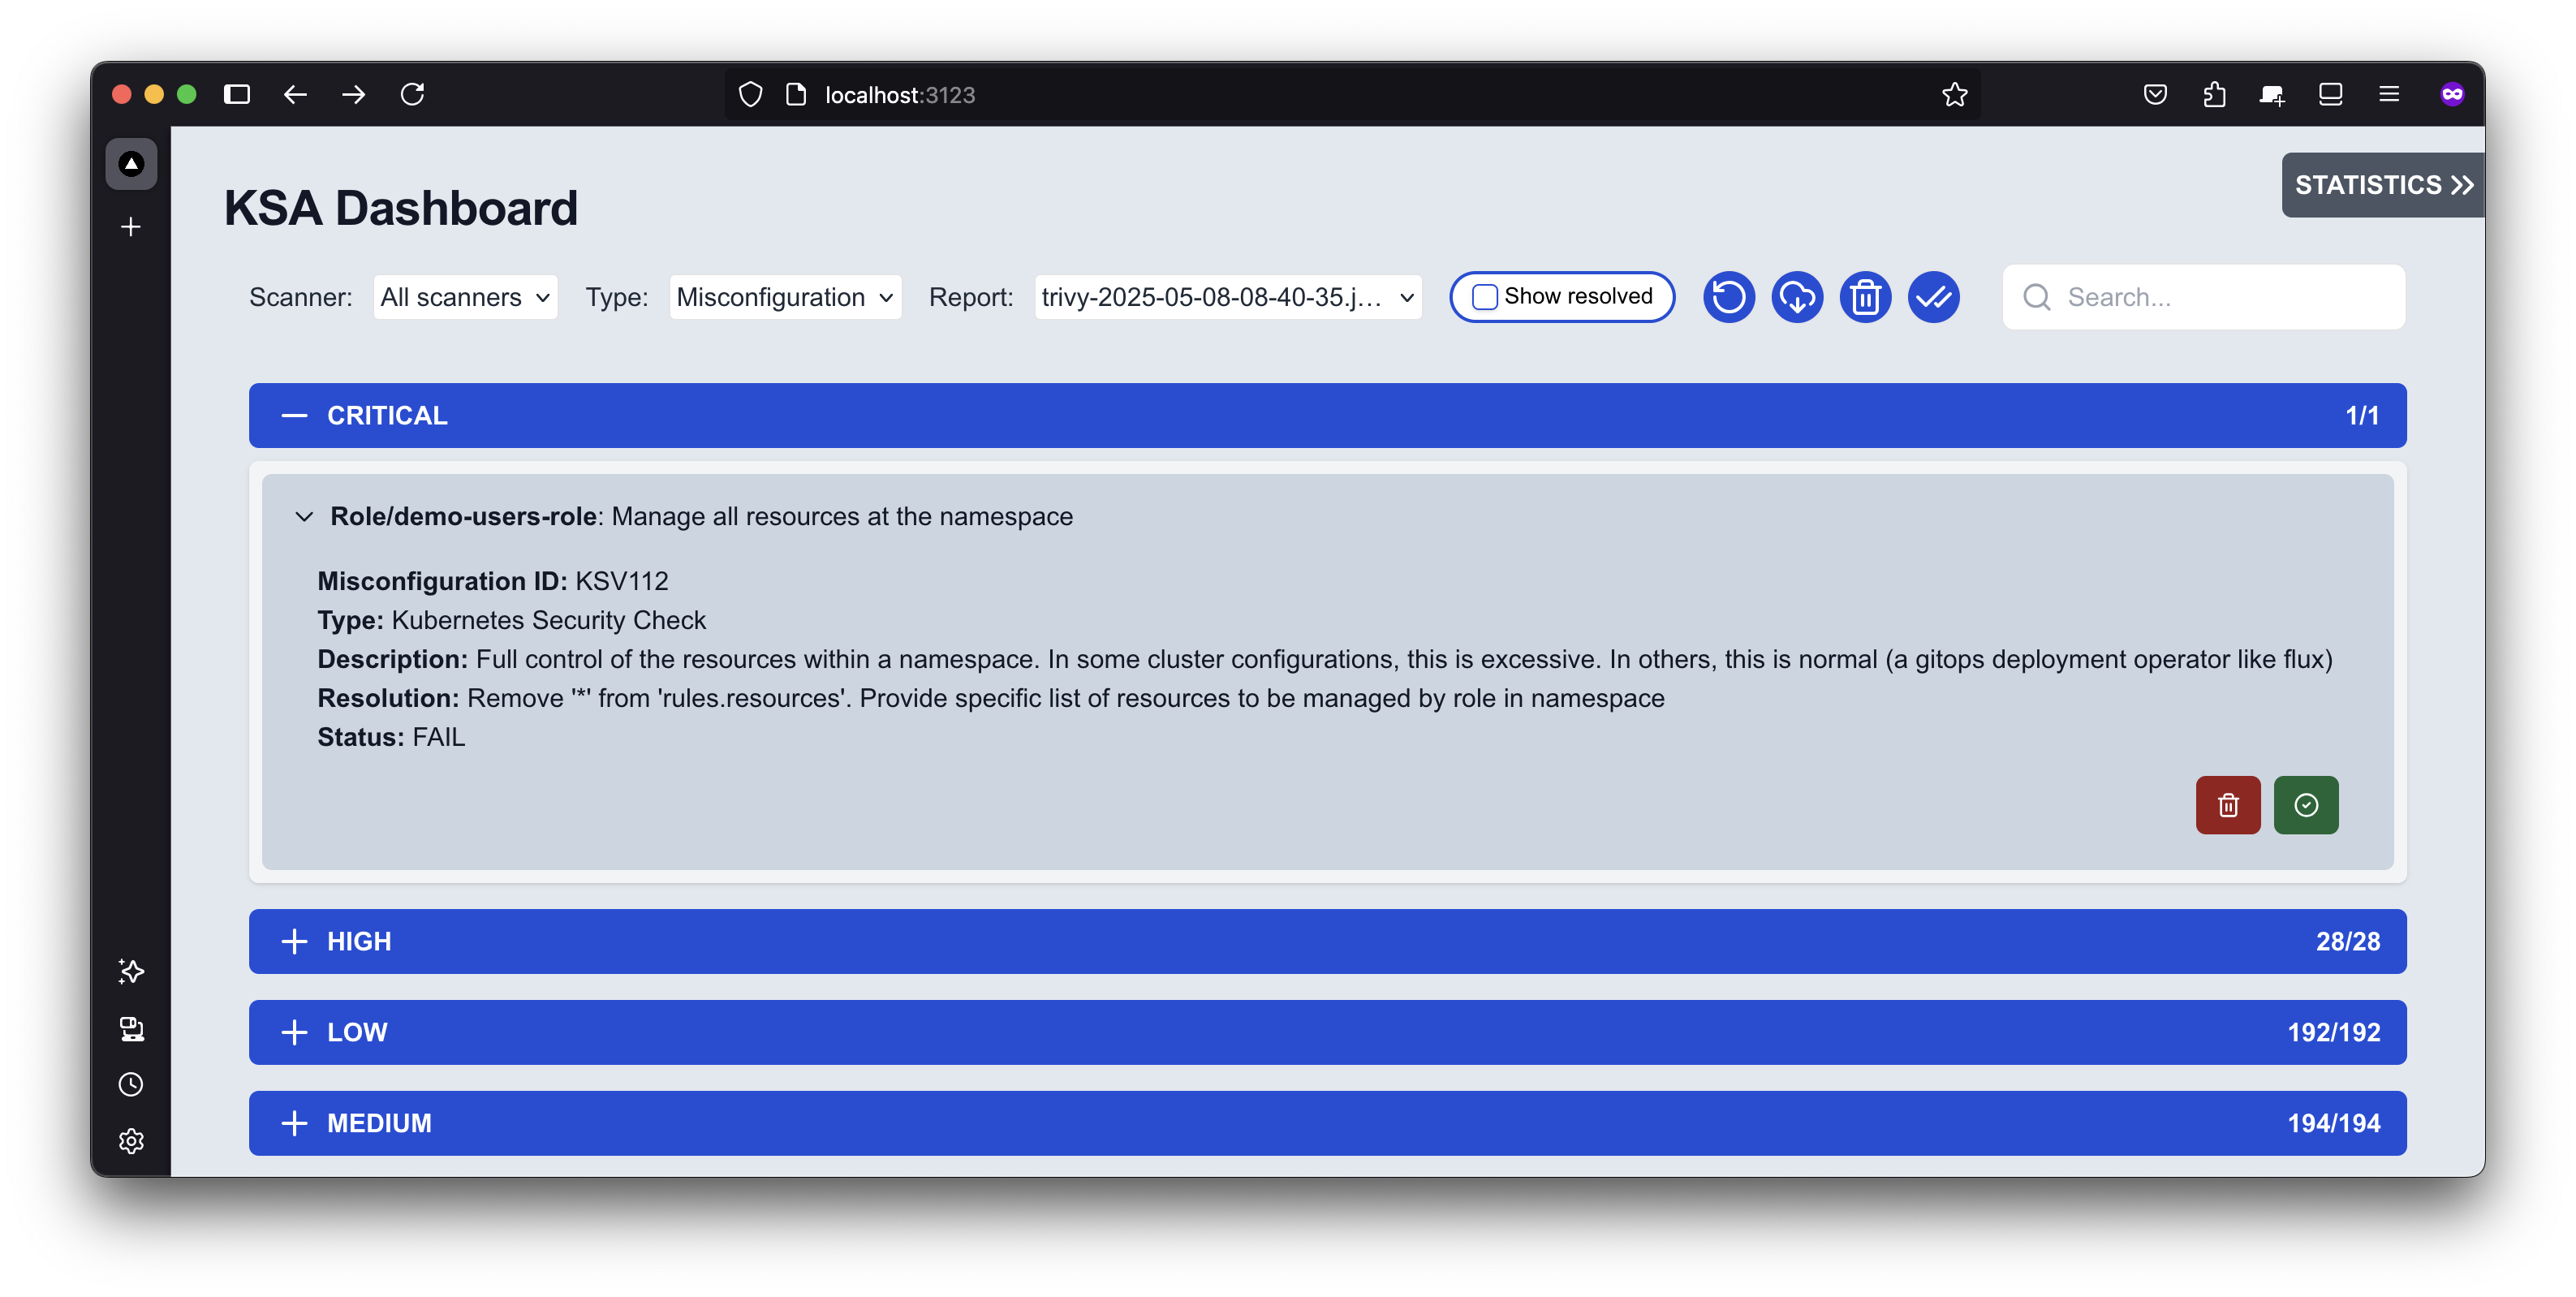
\includegraphics[width=0.9\textwidth]{images/ksa-dashboard-ui.png}
        \caption{User interface of the KSA dashboard.}
		\label{img:ksa-dashboard-ui}
	\end{center}
\end{figure}

The space below the panel is occupied by the list of the security threats. They are collapsed under different categories. Each item can be then also opened to examine the details, such as misconfiguration identifier, type, description, resolution and status. Item titles usually also include the target resource, where the misconfiguration was found.

In the top right corner of the dashboard is a \textbf{STATISTICS} button that provides some information on the most recent scan results in graphical format as shown below in Fig~\ref{img:ksa-dashboard-statistics}.

\begin{figure}[!hbt]
	\begin{center}
		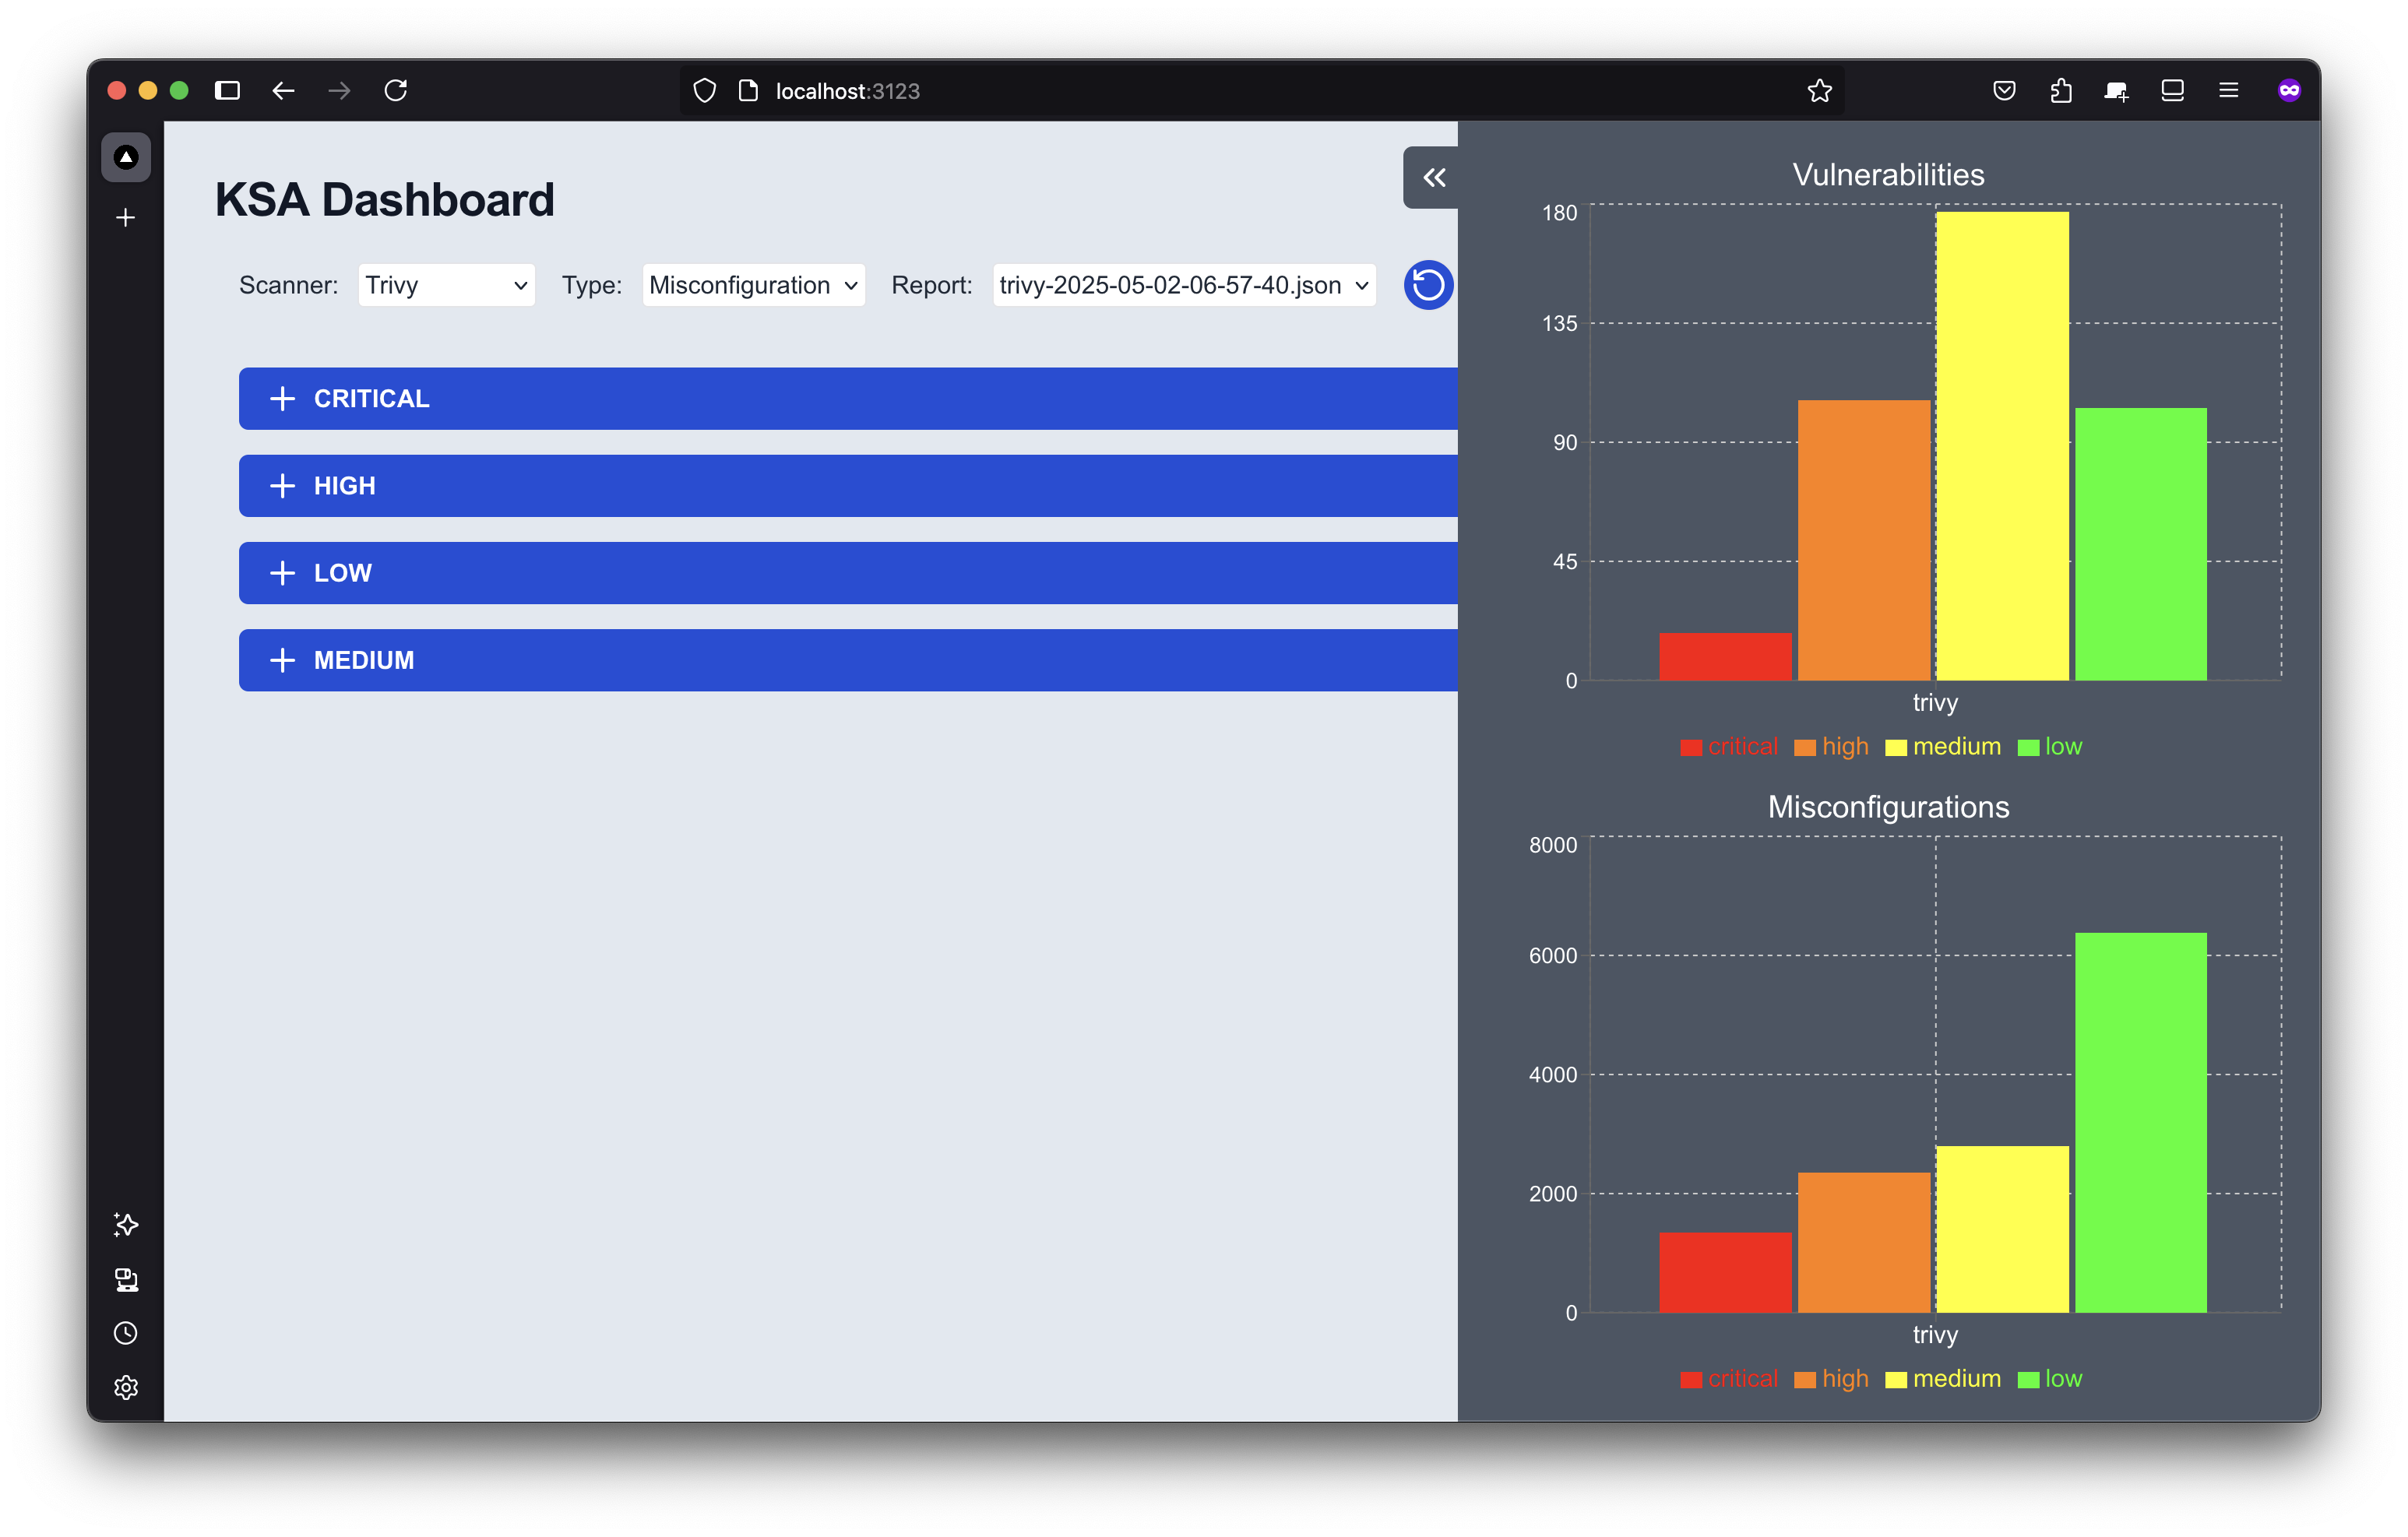
\includegraphics[width=0.9\textwidth]{images/ksa-dashboard-statistics.png}
        \caption{Statistics on the KSA dashboard.}
		\label{img:ksa-dashboard-statistics}
	\end{center}
\end{figure}
\section{Build and Deployment}
\label{sec:build-and-deployment}

Each of the components of the dashboard has a separate Dockerfile, which allows us to containerize the application. Some of the scanners, which do not have a publicly available Docker image, have to be containerized separately. For instance, we build Prowler image on a Python base as shown on the Listing~\ref{lst:prowler-dockerfile}.

\begin{lstlisting}[language=Dockerfile, caption={[Dockerfile definition of Prowler image] Dockerfile definition of Prowler image.}, label={lst:prowler-dockerfile}]
    FROM python:3.12-slim

    RUN pip install prowler
    
    CMD ["prowler"]    
\end{lstlisting}

In order to make it easier to build different components of the application, we define a Bash script that does all of the work for us.

Deployment of the whole application is done via the Helm Chart. It defines all of the Kubernetes resources for the application that are deployed inside the cluster. The deployment can be configured using \lstinline{values.yaml} file, that defines the Helm values, which are then substituted into the Helm templates. Installation is done with 
\begin{center}
    \lstinline{helm -n ksa upgrade --install ksa .}
\end{center} 
command, that creates Deployments, StatefulSet, Services and PVCs. There are also \lstinline{reinstall.sh} and \lstinline{redeploy.sh} Bash scripts defined to automate the installation and redeployment processes, respectively. Listing~\ref{lst:ksa-kubernetes-resources} shows the workloads created by the Helm chart and the Jobs created by the dashboard itself.

When a new scanner is added to the dashboard, the only thing we need to do from the deployment perspective is to define an additional PVC that would hold the reports from the new scanner and mount it to the Parser pod. While it is only a copy-pasting of a few lines, this requires some basic knowledge of Helm. Additional knowledge of Docker would be necessary if an extra image is required for the new scanner.

\begin{lstlisting}[language=CustomBash, caption={[Kubernetes workloads for the KSA Dashboard] Kubernetes workloads for the KSA Dashboard.}, label={lst:ksa-kubernetes-resources}]
$ k get deployments,sts,jobs,pods

NAME                           READY UP-TO-DATE AVAILABLE AGE
deployment.apps/ksa-aggregator 1/1   1          1         2d21h
deployment.apps/ksa-dashboard  1/1   1          1         2d21h
deployment.apps/ksa-parser     1/1   1          1         2d21h

NAME                      READY AGE
statefulset.apps/postgres 1/1   2d21h

NAME                        STATUS   COMPLETIONS DURATION AGE
job.batch/kube-bench-runner Complete 1/1         44s      2d21h
job.batch/prowler-runner    Complete 1/1         4s       2d21h
job.batch/trivy-runner      Complete 1/1         3m20s    2d11h

NAME                                READY STATUS    RESTARTS AGE
pod/ksa-aggregator-7d79b846d5-xzpgt 1/1   Running   0        2d21h
pod/ksa-dashboard-5bd4767cdd-q7ksg  1/1   Running   0        2d21h
pod/ksa-parser-79b55cdf7d-npdjp     1/1   Running   0        2d21h
pod/kube-bench-runner-948bd         0/1   Completed 0        2d21h
pod/postgres-0                      1/1   Running   0        2d21h
pod/prowler-runner-rpdn4            0/1   Completed 0        2d21h
pod/trivy-runner-qp5dw              0/1   Completed 0        2d11h
\end{lstlisting}